%%========================================================================
%% LaTeX scriptiesjabloon
%%========================================================================
%%========================================================================
%% Preamble
%%========================================================================

\documentclass[pdftex,a4paper,12pt,twoside]{report}

\usepackage{color}					 % kleur voor syntax highlighting
\usepackage{caption}
\usepackage{subcaption}
\usepackage[utf8]{inputenc}  % Accenten gebruiken in tekst (vb. � ipv \'e)
\usepackage{amsfonts}        % AMS math packages: extra wiskundige
\usepackage{amsmath}         %   symbolen (o.a. getallen-
\usepackage{amssymb}         %   verzamelingen N, R, Z, Q, etc.)
\usepackage[UKenglish]{babel}    % Taalinstellingen: woordsplitsingen,
                             %  commando's voor speciale karakters
                             %  ("dutch" voor NL)
                                                         %  ("UKenglish" voor brits engels)
\usepackage{eurosym}         % Euro-symbool �
\usepackage{graphicx}        % Invoegen van tekeningen
\usepackage[pdftex,bookmarks=true]{hyperref}
                             % PDF krijgt klikbare links & verwijzingen,
                             %  inhoudstafel
\usepackage{listings}        % Broncode mooi opmaken
\usepackage{multirow}        % Tekst over verschillende cellen in tabellen
\usepackage{rotating}        % Tabellen en figuren roteren
\usepackage{natbib}          % Betere bibliografiestijlen
\usepackage{fancyhdr}        % Pagina-opmaak met hoofd- en voettekst
\usepackage{footnote}
\usepackage{parskip}
\usepackage{longtable}			 % For tables longer than one page


% paragrafen zonder indentatie, en op andere lijn
\setlength{\parindent}{0pt }
\setlength{\parskip}{12pt plus 1pt minus 1pt}


\definecolor{dkgreen}{rgb}{0,0.6,0}
\definecolor{gray}{rgb}{0.5,0.5,0.5}
\definecolor{mauve}{rgb}{0.58,0,0.82}
\definecolor{darkgray}{rgb}{0.662745,0.662745,0.662745}
\definecolor{black}{rgb}{0,0,0}
\definecolor{lightgray}{rgb}{.9,.9,.9}
\definecolor{darkgray}{rgb}{.4,.4,.4}
\definecolor{purple}{rgb}{0.65, 0.12, 0.82}
\definecolor{darkblue}{rgb}{0.0,0.0,0.6}
\definecolor{cyan}{rgb}{0.0,0.6,0.6}


%%---------- Layout ------------------------------------------------------
\newcommand{\includecode}[2][c]{\lstinputlisting[caption=#2, escapechar=]{#2}}

% hoofdingen, enz.
\pagestyle{fancy}

% lijn, wordt gebruikt in titelpagina
\newcommand{\HRule}{\rule{\linewidth}{0.5mm}}

% Leeg blad
\newcommand{\emptypage}
{
	\newpage
	\thispagestyle{empty}
	\mbox{}
	\newpage
}
 
% Gebruik een schreefloos lettertype ipv het "oubollig" uitziende
% Computer Modern
\renewcommand{\familydefault}{\sfdefault}     

% Commando voor invoegen Java-broncodebestanden (dank aan Niels Corneille)
% Gebruik: \codefragment{source/MijnKlasse.java}{Uitleg bij de code}
\newcommand{\codefragmentjava}[2]
{ \lstset{%
  language=java,
  breaklines=true,
  float=th,
  caption={#2},
  basicstyle=\scriptsize,
  frame=single
}
\lstinputlisting{#1}}


\lstset{frame=tb,
  language=Java,
  aboveskip=3mm,
  belowskip=3mm,
  showstringspaces=false,
  columns=flexible,
  basicstyle={\small\ttfamily},
  numbers=left,
  numberstyle=\footnotesize,
  keywordstyle=\color{blue},
  commentstyle=\color{dkgreen},
  stringstyle=\color{mauve},
  breaklines=true,
  breakatwhitespace=true
  tabsize=3,
	captionpos=b,
	extendedchars=true
}

\lstdefinelanguage{JavaScript}
{
  keywords={typeof, new, true, false, catch, function, return, null, catch, switch, var, if, in, while, do, else, case, break},
  keywordstyle=\color{blue}\bfseries,
  ndkeywords={class, export, boolean, throw, implements, import, this},
  ndkeywordstyle=\color{darkgray}\bfseries,
  identifierstyle=\color{black},
  sensitive=false,
  comment=[l]{//},
  morecomment=[s]{/*}{*/},
  commentstyle=\color{purple}\ttfamily,
  stringstyle=\color{red}\ttfamily,
  morestring=[b]',
  morestring=[b]"
}

\lstdefinelanguage{XML}
{
  basicstyle=\ttfamily\color{darkblue}\bfseries,
  morestring=[b]",
  morestring=[s]{>}{<},
  morecomment=[s]{<?}{?>},
  stringstyle=\color{black},
  identifierstyle=\color{darkblue},
  keywordstyle=\color{cyan},
  morekeywords={xmlns,version,type}% list your attributes here
}


\lstdefinelanguage{CSS}
{
	alsodigit={-},
	ndkeywords={@import, @media, @page, @font-face, @charset, @namespace, @viewport, @-ms-viewport, @-o-viewport, @-moz-viewport, @-webkit-viewport, th},
  ndkeywordstyle=\color{darkgray}\bfseries,
  morekeywords={accelerator,azimuth,background,background-attachment,
    background-color,background-image,background-position,
    background-position-x,background-position-y,background-repeat,
    behavior,border,border-bottom,border-bottom-color,
    border-bottom-style,border-bottom-width,border-collapse,
    border-color,border-left,border-left-color,border-left-style,
    border-left-width,border-right,border-right-color,
    border-right-style,border-right-width,border-spacing,
    border-style,border-top,border-top-color,border-top-style,
    border-top-width,border-width,bottom,caption-side,clear,
    clip,color,content,counter-increment,counter-reset,cue,
    cue-after,cue-before,cursor,direction,display,elevation,
    empty-cells,filter,float,font,font-family,font-size,
    font-size-adjust,font-stretch,font-style,font-variant,
    font-weight,height,ime-mode,include-source,
    layer-background-color,layer-background-image,layout-flow,
    layout-grid,layout-grid-char,layout-grid-char-spacing,
    layout-grid-line,layout-grid-mode,layout-grid-type,left,
    letter-spacing,line-break,line-height,list-style,
    list-style-image,list-style-position,list-style-type,margin,
    margin-bottom,margin-left,margin-right,margin-top,
    marker-offset,marks,max-height,max-width,min-height,
    min-width,-moz-binding,-moz-border-radius,
    -moz-border-radius-topleft,-moz-border-radius-topright,
    -moz-border-radius-bottomright,-moz-border-radius-bottomleft,
    -moz-border-top-colors,-moz-border-right-colors,
    -moz-border-bottom-colors,-moz-border-left-colors,-moz-opacity,
    -moz-outline,-moz-outline-color,-moz-outline-style,
    -moz-outline-width,-moz-user-focus,-moz-user-input,
    -moz-user-modify,-moz-user-select,orphans,outline,
    outline-color,outline-style,outline-width,overflow,
    overflow-X,overflow-Y,padding,padding-bottom,padding-left,
    padding-right,padding-top,page,page-break-after,
    page-break-before,page-break-inside,pause,pause-after,
    pause-before,pitch,pitch-range,play-during,position,quotes,
    -replace,richness,right,ruby-align,ruby-overhang,
    ruby-position,-set-link-source,size,speak,speak-header,
    speak-numeral,speak-punctuation,speech-rate,stress,
    scrollbar-arrow-color,scrollbar-base-color,
    scrollbar-dark-shadow-color,scrollbar-face-color,
    scrollbar-highlight-color,scrollbar-shadow-color,
    scrollbar-3d-light-color,scrollbar-track-color,table-layout,
    text-align,text-align-last,text-decoration,text-indent,
    text-justify,text-overflow,text-shadow,text-transform,
    text-autospace,text-kashida-space,text-underline-position,top,
    unicode-bidi,-use-link-source,vertical-align,visibility,
    voice-family,volume,white-space,widows,width,word-break,
    word-spacing,word-wrap,writing-mode,z-index,zoom},
  morestring=[s]{:}{;},
	moredelim=[is][\color{black}\bfseries]{@*}{*@},
	moredelim=[is][\color{mauve}\bfseries]{@.}{.@},
	moredelim=[is][\color{blue}\bfseries]{@~}{~@},
	moredelim=[is][\color{red}\bfseries]{@�}{�@},
  sensitive,
  morecomment=[s]{/*}{*/}
}

%%---------- Documenteigenschappen ---------------------------------------
%% Vul dit aan met je eigen info:

% Je eigen naam
\newcommand{\studenta}{Kenzo Clauw}
\newcommand{\studentb}{Axl Fran\c{c}ois}
\newcommand{\studentc}{Lowie Huyghe}
\newcommand{\studentd}{Sander Trypsteen}
\newcommand{\studente}{Jelle Verreth}

% De naam van je stage-/bachelorproefbegeleider
%\newcommand{\begeleider}{} 

% De naam (én firma/organisatie) van je mentor/promotor
% Laat in commentaar indien niet van toepassing
%\newcommand{\mentor}{Jan Janssen, ACME Inc.}

% De titel van je scriptie/stageverslag
\newcommand{\titel}{VOP Project Dossier}

% Ondertitel
\newcommand{\ondertitel}{ Stambomen}

% Datum van indienen
\newcommand{\datum}{XX XXXX 2014}

% Academiejaar
\newcommand{\academiejaar}{2013-2014}

%%========================================================================
%% Inhoud document
%%========================================================================

\begin{document}

%%---------- Front matter ------------------------------------------------
%% Het voorblad - Hier moet je in principe niets wijzigen.

\begin{titlepage}
\begin{center}

\includegraphics[width=4cm]{images/logo.png}\\[.5cm]
Master of Science Industrial Science : Informatics\\
Academic year \academiejaar

\vfill

\HRule \\[0.4cm]
{ \huge \bfseries \titel}\\[0.4cm]
\HRule \\[0.4cm]

{\Large \ondertitel}\\[0.4cm]

Submitted on \datum

\vfill

% Studenten en begeleiders
\begin{minipage}{0.49\textwidth}
\begin{flushleft}
\emph{Student\ifdefined\studentb s\fi :}\\
\studenta \\
\studentb \\
\studentc \\
\studentd \\
\studente
\par
\end{flushleft}
\end{minipage}
\begin{minipage}{0.49\textwidth}
\begin{flushright}
%\emph{Tutor:}\\ \begeleider\\
%\ifdefined\mentor \emph{Mentor:}\\ \mentor \fi
\end{flushright}
\end{minipage}

\end{center}

\end{titlepage}

% Schutblad

\emptypage

% Herhaling titelblad

\begin{titlepage}
\begin{center}
Master of Science Industrial Science : Informatics\\
Academic year \academiejaar

\vfill

\HRule \\[0.4cm]
{ \huge \bfseries \titel}\\[0.4cm]
\HRule \\[0.4cm]

{\Large \ondertitel}\\[0.4cm]

Submitted on \datum

\vfill

% Studenten en begeleiders
\begin{minipage}{0.49\textwidth}
\begin{flushleft}
\emph{Student\ifdefined\ \fi :}\\
\studenta \\
\studentb \\
\studentc \\
\studentd \\
\studente
%\ifdefined\studentb \studentb \fi\par
\end{flushleft}
\end{minipage}
\begin{minipage}{0.49\textwidth}
\begin{flushright}
%\emph{Tutor:}\\ \begeleider\\
%\ifdefined\mentor \emph{Mentor:}\\ \mentor \fi
\end{flushright}
\end{minipage}

\end{center}

\end{titlepage}

%% Inhoudstafel
\abstract


\tableofcontents

\chapter{Voorwoord}\label{ch:preface}

\paragraph{}
Dit projectdossier is een schriftelijk neerslag van onze prestaties voor het vakoverschrijvend project\footnote{VOP}. Hierin bespreken we de verschillende facetten van ons project. 
Allereest zullen wij beginnen met de opdracht voor te stellen en ze te situeren. Hierbij zullen we proberen van een zo volledig mogelijk overzicht te geven van alle technische en niet-technische onderdelen. Vervolgens krijgt u meer uitleg over de manier waarop onze takenverdeling tot stand komt en het volledig overzicht van onze takenverdeling.
Daarna bespreken we de analyse van het project aan de hand van enkele diagrammen en use cases. Vervolgens lichten we enkele belangerijke aspecten van ons project toe. We gaan hier zowel in op ontwerpbeslissingen als op implementatiekeuzes. Dan komen we aan de kwaliteitscontrole voldoet onze applicatie aan de fucntionele en niet-functionele veresiten zoals deze zijn opgesteld door de klant? Uiteraard zijn er in elk project wel problemen en we zullen het niet na laten om deze te bespreken. Als voorlaatste geven we nog even onze visie op het verdere verloop van de applicatie. Waar kan het beter, welke uitbreidingen zijn mogelijk. Ten slotte eindigen we met een nabeschouwing en ons besluit over het VOP.
\chapter{Introductie en situering}\label{ch:introduction}

\section{Introductie}
In deze paper kan u meer informatie vinden rond ons vop. Het onderwerp zoals u wellicht al gelezen hebt op het titel blad zijn stambomen. Het woord stambomen kan in verschillende contexten bekeken worden. We beperken ons echter enkel tot de genealogie. In genealogie zitten twee Griekse woorden verborgen namelijk Genea en Logos. Genea staat voor afkomst of afstamming en logos betekent wetenschap of kennis. 
Dus we bestuderen hier de afkomst, afstamming van een persoon.
In dit project zijn er echter twee bepererkingen:
\paragraph{}
Zonder dieper in te gaan op het onderwerp genealogie willen ook nog melden dat in dit project we ons slechts zullen beperken tot natuurlijk mogelijke afstammelingen. Hieronder verstaan wij dat er enkel man - vrouw relaties mogelijk zijn. We houden dus geen rekening met man - man of vrouw - vrouw relaties die dan kinderen zouden hebben.

\paragraph{}
Verder houden we ook geen rekening met de onderlinge relaties tussen echtparen. Op zich zijn dat onze zaken niet maar wanneer een persoon een buitenechtelijke kind heeft dan zal hij dat niet kunnen invoeren in ons programma. Hieronder vallen dus ook half-broers of half-zussen. Deze zullen niet weergegeven worden in ons stamboom overzicht.

\paragraph{}
Nu de scope van de opdracht duidelijker is kunnnen ingaan op wat er gevraagd is. Het is de bedoeling om een applicatie te maken waar een gebruiker stambomen kan ingeven en bekijken. De gebruiker moet deze stambomen kunnen raadplegen via een website  en de bomen worden ingegeven via een desktop applicatie. Verder moet de gebruiker ook zijn bomen kunnen delen met zijn vrienden zowel binnen de applicatie als op sociale netwerk sites. Voor dit project zullen we ons qua sociale netwerk sites beperken tot Facebook.

\section{Technische}
\paragraph{}
We hebben op 10/02/2014 de inleidende presentatie van het vop gekregen. Hierin werden een aantal vereisten uitgelegd. Deze vereisten staan uitgebreid beschreven in VOP: de richtlijnen \footnote{ADD REFERENCE}. De belangrijkste hierin zijn dat er een docent de rol van klant zal spelen. Er zullen afspraken moeten worden gemaakt met de klant over wat al dan niet mogelijk is. Wat er moet gerealiseerd worden? We kwamen ook te weten dat het project in Java moest geschreven worden. Verder moest dit gebeuren door aan de hand van een drielagen architectuur. 

\paragraph{Presentatie laag}
Deze laag bestond uit twee onderdelen namelijk een Java Desktop Client gemaakt in Java Swing en een website (HTML5, Javascript) die gebruikt maakt van Java Servlets. De nadruk uiteraard ligt hier bij het scheiden van onze logica van de presentatie.

\paragraph{Domein logica}
Hierbij was het de bedoeling om een REST-service in Java op te zetten waarvan de presentatie gebruik kan maken. We hebben hier van in het begin gekozen om Jersey te gebruiken.

\paragraph{Data tier}
Een relationele databank ging in staan voor de persistentie van onze gegevens. De databank die ons aangeboden werd door UGent is MySQL. We mochten in deze opdracht geen gebruik maken van ORM-tools\footnote{Object-Relational Mapping zoals Hibernate.}. 

\section{Situering}
\paragraph{}
WAT?

\chapter{Taak-verdeling}

\section{Methodologie}
\paragraph{}
Tijdens dit project zullen we gebruik maken van Scrum. Hierbij verdelen we het project in drie sprints. Aan het begin van elke sprint zitten we samen om te bespreken welke features we graag zouden opnemen. Hoe lang een bepaalde feature duurt om uit te werken. Na deze bespreking maken we een afspraak bij de klant.

\paragraph{}
Met de klant bespreken we dan welke features voor ons mogelijk zijn en welke features voor de klant noodzakelijk zijn. Hieruit volg een contract, alle features die we tijdens een bepaalde sprint zullen realiseren.

\paragraph{}
Op het einde van de sprint kijken we dan welke features we gerealiseerd hebben en welke niet. Dankzij deze methode kunnen we inschatten of we tijdens het project moeten bijsturen. Het kan zijn dat we niet alle features gerealiseerd hebben dan moeten we harder werken tijdens de volgende sprint.

\paragraph{}
Tijdens elke sprint krijgen we van de docenten een voorgestelde lijst met features.

\section{Sprint 1}

\subsection{Kenzo Clauw}

\subsection{Axl François}

\subsection{Lowie Huyghe}

\subsection{Sander Trypsteen}

\subsection{Jelle Verreth}

\section{Sprint 2}

\subsection{Kenzo Clauw}

\subsection{Axl François}

\subsection{Lowie Huyghe}

\subsection{Sander Trypsteen}

\subsection{Jelle Verreth}

\section{Sprint 3}

\subsection{Kenzo Clauw}

\subsection{Axl François}

\subsection{Lowie Huyghe}

\subsection{Sander Trypsteen}

\subsection{Jelle Verreth}

\section{Overzicht}

\chapter{Analyse}

\chapter{Interresantee Ontwerpbeslissingen}

\chapter{Interessante Implementatiekeuzes}
\section{Bibliotheken}
\subsection{Jersey}

Jersey is een JAX-RS referentie-implementatie die een eigen API aanbied door de JAX-RS toolkit uit te breiden met extra functies en hulpprogramma's om op een eenvoudige manier RESTful Webservices en client development aan te bieden.
JAX-RS : Java API voor REST Web Services biedt ondersteuning bij het creëren van web services volgens het Representational State Transfer (REST) pattern.
REST is een pattern die beschrijft hoe resources geadresseerd en gebruikt kunnen worden.Een resource kan aangesproken worden dankzij een gemeenschappelijke interface op basis van de HTTP standaard methodes.
Een REST server zorgt ervoor dat de client een verbinding kan maken om de resources op te halen en te wijzigen. REST wordt veel gebruikt voor het bouwen van webservices en noemen we respectievelijk RESTful Webservices.
Voor de applicatie hebben we gebruik gemaakt van Jersey die zorgt voor de REST server en een REST client.


\subsection{Swagger Jersey}
Swagger is een specificatie en compleet uitvoeringskader voor het bescrijven, het produceren , consumeren en visualiseren van REST webservices. Het doel van Swagger om client en documentatie systemen de mogelijkheid te geven op hetzelfde tempo te werken als de server. De documentatie van de methoden,paremeters en modellen zijn nauw geintegreerd in de server-code, waardoor de API's altijd gesynchroniseerd zijn.

Door gebruik te maken van Swagger kunnen clients diensten consumeren en toegang tot de server code zonder in aanraking te komen de implementatie van de server.
De interface van het framework zorgt ervoor dat er interactie mogelijk is  met de API in een sandbox omgeving.
Swagger ondersteunt JSON en XML en zal in de toekomst ook beschikbaar zijn in andere formaten. 





\subsection{SLF4J}
SLF4J is een Java logging api die gebruik maakt van een facade pattern, dit is een software design pattern die gebruikt wordt in object-oriented programming om een complex systeem voor te stellen als een interface.
De facade pattern is ideaal bij het werken met een groot aantal onderling afhankelijke klassen of klassen die meerdere methoden gebruiken , vooral wanneer deze te ingewikkeld zijn om te gebruiken of moeilijk te begrijpen.
De onderliggende logging backend van SLFJ4J wordt bepaald op runtime door het toevegen van de gewenste binding aan het classpath ( java.util.logging).
Om gebruik te maken van SLF4J moet je de slf4j-api-1.7.7.jar en slf4j-simple-1.7.7.jar plaatsen in de classpath van het project.
Bij het volgende voorbeeld roepen we de loggerfactory op om dan vervolgens het toevoegen van een persoon te registeren :

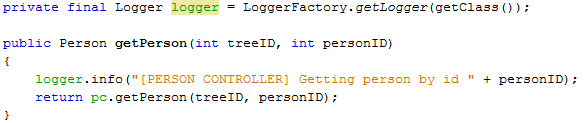
\includegraphics{images/logger.png}\\


\subsection{Junit}
JUnit is een unit testing framework voor Java die gebruikt wordt in test-driven development die deel uit maak van xUnit.
Een unit test is een stukje code die een specifieke functionaliteit uitvoert om de code testen. Het percentage van de code die wordt getest door unit tests wordt meestal de test coverage genoemd.
Een unit test richt zich op een kleine eenheid van de code , bv een methode of een klasse.


\subsection{Gedcom}

GEDCOM is een speciaal tekstformaat die ontwikkeld is door de Kerk van Jezus Christus van de Heiligen der Laatste Dagen en is bedoeld als standaard voor communicatie tussen de Kerk en personen die genealogische data aanleveren.
Dit formaat heeft zich nu ontwikkeld tot de standaard voor gegevensuitwisseling tussen de meeste genealogische programma's en systemen.

Stel dat we in de applicatie een persoon toevoegen dan zouden deze gegevens in een GEDCOM als volgt voorgesteld worden :

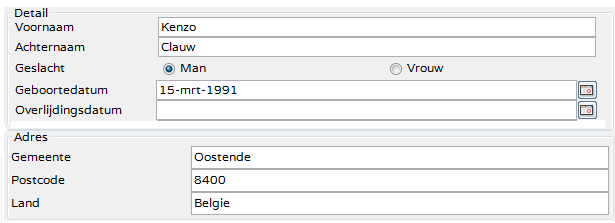
\includegraphics{images/gedcom.png}\\

Het eerste deel bevat de header met de gebruikte versie,character encoding (ANSEl,UNICODE of ASCII) als de belangrijkste informatie.


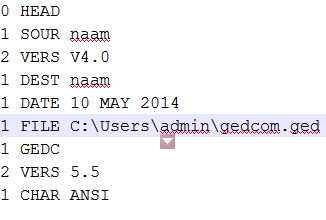
\includegraphics{images/gedcomheader.png}\\

Het tweede deel bevat informatie over de personen.

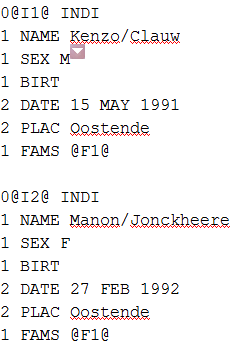
\includegraphics{images/gedcomperson.png}\\

Het laatste deel bevat de relaties tussen personen met TRLR die het bestand afsluit.

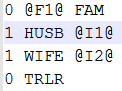
\includegraphics{images/gedcomrelaties.png}\\

\subsection{Gedcom4j}
Gedcom4j is een gratis open-source Java library voor het laden ( parsing ) en opslaan van gegevens in Gedcom genealogie 5.5 of 5.51 bestanden naar een Java-object hiërarchie.

Om gebruik te maken van Gedcom4j moet je de gedcom4j.jar plaatsen in de classpath van het project.

Om toegang tot gegevens te verkrijgen maak je gebruik van de properties binnen de gp.gedcom structure waarbij de personen voorgesteld worden door het object Individual en de relaties door Family.

Laden van een gedcom bestand :

GedcomParser gp = new GedcomParser();
gp.load("sample/TGC551.ged");

Om de personen te overlopen  :

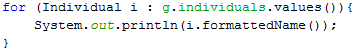
\includegraphics{images/gedcomindividual.png}\\

Om de relaties met kinderen te overlopen :

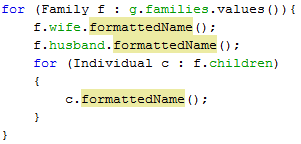
\includegraphics{images/gedcomfamily.png}\\

\subsection{Sardine}
\subsection{RestFB}
\subsection{JCalendar}
\subsection{Abego TreeLayout}
ABEGO TreeLayout is een Efficiënt en aanpasbare Boom Layout algoritme voor Java.
De TreeLayout creëert boom lay-outs voor willekeurige bomen. Het is niet beperkt tot een bepaalde productie of formaat, maar kan worden gebruikt voor elke vorm van tweedimensionale tekening. Voorbeelden zijn Swing gebaseerde componenten, SVG-bestanden, en nog veel meer.

Om de Treelayout te gebruiken moet je een instantie van de klasse TreeLayout voorzien van de knooppunten van de boom inclusief zijn kinderen samen met de hoogte tussen verchillende niveaus.

Eigenschappen :
Op basis van deze informatie zorgt de TreeLayout voor een compacte layout met een overzichtelijke boom.

De indeling toont de hiërarchische structuur van de boom, namelijk de y-coördinaat van een knooppunt wordt bepaald door het niveau.

De randen kruisen elkaar niet en de nodes op hetzelfde niveau hebben een minimale horizontale afstand.
De volgorode van de kinderen van een knooppunt wordt weergegeven in de tekening.

Het algoritme werkt symmetrisch, dat wil zeggen de tekening van de weerspiegeling van een boom is het gereflecteerde tekening van de oorspronkelijke boom


Om gebruik te maken van de Abego TreeLayout moet je de org.abego.treelayout.core.jar(de TreeLayout algoritme kern) en org.abego.treelayout.netbeans.jar( gebruikt  van de NetBeans visuele API ) plaatsen in de classpath van het project.


\subsection{Java FX}

\chapter{Kwaliteitscontrole}

Om de kwaliteit van onze applicatie te garanderen wordt er gebruik gemaakt van Test-driven development die een onderdeel is van agile softwareontwikkeling.

Hoe werkt Test-driven development?

Voor dat er code geschreven wordt maak je eerst een geautomatiseerde test waarbij je rekening moet houden met alle mogelijkheden van invoer , errors en uitvoer. Op deze manier moet je nog geen rekening houden met code.
De eerste keer dat een test uitgevoerd wordt moet deze een error produceren omdat er nog geen code aanwezig is.
Na het afwerken van de test is het de bedoeling om op basis van de tests code te schrijven.
Eens de code met succes de verschillende testen kan doorstaan kun je bepaalde bugs uit je applicatie al uitsluiten.

Wij hebben ervoor gekozen om aan de hand van JUnit de opgestellende use cases om uitgebreid te testen in onze applicaite aan de hand van een JUnit test suite.

Wat moet er getest worden?

In het algemeen is het veilig om bepaalde methoden zoals getters en setters die gewoon waarden oproepen of toewijzen te negeren. Het schrijven van tests hiervoor is tijdrovend en zinloos omdat je op deze manier de Java Virtual Machine zou testen waarvoor er al testen voorzien zijn.







\chapter{Gekende problemen}

\chapter{Verbeterpunten en uitbreidingsmogelijkheden}

\chapter{Nabeschouwing en besluit}


%%%%%%%%%%%%%%%%%%%%%%%%%%%%%%%%%%%%%%%%%%%%%%%%%%%%%%%%%%%%%
%% BIBLIOGRAPHY AND OTHER LISTS
%%%%%%%%%%%%%%%%%%%%%%%%%%%%%%%%%%%%%%%%%%%%%%%%%%%%%%%%%%%%%
%% A small distance to the other stuff in the table of contents (toc)
\addtocontents{toc}{\protect\vspace*{\baselineskip}}

%% The Bibliography
%% ==> You need a file 'literature.bib' for this.
%% ==> You need to run BibTeX for this (Project | Properties... | Uses BibTeX)
%\addcontentsline{toc}{chapter}{Bibliography} %'Bibliography' into toc
%\nocite{*} %Even non-cited BibTeX-Entries will be shown.
%\bibliographystyle{alpha} %Style of Bibliography: plain / apalike / amsalpha / ...
%\bibliography{literature} %You need a file 'literature.bib' for this.

%% The List of Figures
\clearpage
\addcontentsline{toc}{chapter}{List of Figures}
\listoffigures

%% The List of Tables
\clearpage
\addcontentsline{toc}{chapter}{List of Tables}
\listoftables

%%%%%%%%%%%%%%%%%%%%%%%%%%%%%%%%%%%%%%%%%%%%%%%%%%%%%%%%%%%%%
%% APPENDICES
%%%%%%%%%%%%%%%%%%%%%%%%%%%%%%%%%%%%%%%%%%%%%%%%%%%%%%%%%%%%%

\appendix
%\input{FileName} %You need a file 'FileName.tex' for this.

\end{document}

